\documentclass[11pt,a4paper]{article}
\usepackage[T1]{fontenc}
\usepackage[utf8]{inputenc}
\usepackage[margin=2cm]{geometry}
\usepackage{booktabs,longtable,array,float,graphicx}
\usepackage{setspace}
\usepackage[colorlinks=true,linkcolor=black,urlcolor=blue,citecolor=black]{hyperref}
\setstretch{1.1}
\setlength{\parindent}{1.2em}
\setlength{\parskip}{0.3em}
\graphicspath{{figures/}{../figures/}}

\begin{document}

\begin{titlepage}
\centering
\IfFileExists{logo.png}{\includegraphics[height=2.5cm]{logo.png}\par}{{\itshape [Insert institution logo here: upload logo.png to the project]}\par}
\vspace{1.5cm}
{\LARGE\bfseries ECG-Based Arrhythmia Classification: A Comparative Study of Classical Machine Learning and Deep Learning Architectures Using Metaheuristic Hyperparameter Optimization\par}
\vspace{1cm}
{\large Deep Learning Mini Project -- Phase 3 (Final Report)\par}
{\large [ICT-4442]\par}
\vspace{1.5cm}
{\large\textbf{Submitted By}\par}
\vspace{0.5cm}
\begin{tabular}{ll}
Tanush Ralhan & 230911564 \\
Pranshu Singh & [registration number] \\
Chinmai & 230911318 \\
\end{tabular}
\vfill
{\large SCHOOL OF COMPUTER ENGINEERING\par}
{\large MANIPAL INSTITUTE OF TECHNOLOGY,\par MANIPAL ACADEMY OF HIGHER EDUCATION\par}
\vspace{0.5cm}
{\large OCTOBER, 2026\par}
\vspace{0.3cm}
{\small Code repository: \url{https://github.com/CHINMAYBHT/Arrhythmia-Detection}\par}
\end{titlepage}

\section*{Abstract}
Automatic classification of heartbeats from the electrocardiogram (ECG) could support continuous cardiac monitoring, but published accuracies are often obtained with train/test splits that mix beats from the same patient. We compare three model families on the MIT-BIH Arrhythmia Database under one patient-independent protocol (the DS1/DS2 record split) and the five AAMI EC57 beat classes: an SVM and a Random Forest on hand-crafted morphology, wavelet and RR-interval features; a 1D convolutional neural network (CNN) on the raw beat window; and a CNN-LSTM that classifies a beat from the sequence of five beats ending at it. We also test whether two metaheuristic optimizers, the Grey Wolf Optimizer (GWO) and the Whale Optimization Algorithm (WOA), tune the CNN's hyperparameters better than a grid search with the same budget. On the 49,697 held-out test beats, the Random Forest achieves both the highest accuracy (0.860) and the highest macro-F1 (0.393), followed by the SVM (macro-F1 0.353); the best deep model, a WOA-tuned CNN, reaches 0.346 and the CNN-LSTM 0.335. All models detect ventricular ectopic beats reasonably well (best F1 0.79), but none reliably detects supraventricular (S) or fusion (F) beats, so macro-F1 stays between 0.32 and 0.39. GWO and WOA found configurations with higher validation scores than grid search, but these gains did not carry over to the test patients: the best tuned CNN (WOA) improves macro-F1 over the untuned CNN by only 0.005. We conclude that, under a strict inter-patient protocol, the choice of model family and tuner matters far less than the limited number of training patients and the class imbalance.

\noindent\textbf{Keywords:} ECG, arrhythmia classification, MIT-BIH, AAMI EC57, inter-patient evaluation, 1D-CNN, CNN-LSTM, Random Forest, SVM, Grey Wolf Optimizer, Whale Optimization Algorithm.

\newpage
\tableofcontents
\newpage

%=====================================================================
\section{Introduction}
Cardiac arrhythmias are disturbances of the heart's rhythm, and some of them are early signs of serious cardiovascular disease. The standard way to detect them is a cardiologist reading an ECG trace. This is slow, depends on the reader, and is not possible for the many hours of signal produced by Holter monitors and wearable devices. Automatic beat classification is therefore a long-studied problem, and the MIT-BIH Arrhythmia Database [1], [2] is its standard benchmark.

Two families of methods dominate the literature. Classical methods compute hand-crafted features from each beat, such as RR intervals, QRS morphology and wavelet coefficients, and train a classifier such as an SVM or a Random Forest on them [12]. Deep learning methods learn the features directly from the raw signal with 1D CNNs [3], [13], [14], and recurrent or hybrid CNN-LSTM networks additionally model the sequence of beats [5], [7], [15]. Many reported accuracies above 95\% are obtained with intra-patient splits, in which beats of the same patient appear in both training and test sets. Under an inter-patient split, where test patients are never seen in training, performance on the minority classes drops sharply [4], [5], [12], [16].

This project compares one model from each family on the same data, split by patient and scored with the same metrics, so that the differences between models can be attributed to the models. As a side experiment, it tests whether two nature-inspired metaheuristic optimizers, GWO [9] and WOA [10], [17], find better CNN hyperparameters than a grid search given the same compute budget, a question that has so far mostly been studied on medical images [11].

%=====================================================================
\section{Literature Review}
The literature relevant to this project falls into four groups: classical feature-based classifiers, convolutional networks, recurrent and hybrid networks, and metaheuristic hyperparameter optimization. Table~\ref{tab:lit} summarises the main papers.

\subsection{Evaluation protocol and classical feature-based methods}
De Chazal, O'Dwyer and Reilly [12] introduced the inter-patient DS1/DS2 split of MIT-BIH that we use and showed that a linear discriminant classifier on morphology and RR-interval features reaches high sensitivity for V beats but much lower performance for S beats on unseen patients. Their work established RR intervals as essential features for the S class, because a supraventricular beat has a nearly normal shape but arrives early. The AAMI EC57 standard [18] defines the five beat classes (N, S, V, F, Q) that we use. Ben Slama et al. [8] showed that an SVM on CNN-extracted features can outperform the CNN alone (97.33\% against 85.52\%), so a classical classifier is not necessarily weaker than a deep network; the outcome depends on the features. Nikandish, He and Haghi [6] fused wavelet, interval and area features and raised the accuracy of difficult beat types considerably. These papers motivate Model 1: an SVM [19] and a Random Forest [20] on morphology, wavelet and RR-interval features. Silva et al. [16] reviewed studies from 2017 to 2024 and found that few follow the inter-patient protocol, which makes published numbers hard to compare. This supports our choice of a single common protocol.

\subsection{Convolutional networks}
Kiranyaz, Ince and Gabbouj [13] showed that a compact 1D-CNN can learn features directly from raw ECG beats, although their best results used a patient-specific training scheme. Acharya et al. [14] trained a 9-layer CNN on MIT-BIH beats and reported 94\% accuracy on an intra-patient split. Khan et al. [3] reported 95.2\% accuracy for five heartbeat classes, but did not state whether their split was patient-independent. Guo, Sim and Matuszewski [4] evaluated DenseNet and GRU models on the inter-patient split and obtained F1 of 61.25 for S beats and 89.75 for V beats, which shows that S remains the hardest class even for deep networks. Model 2 is a 1D-CNN of this kind.

\subsection{Recurrent and hybrid networks}
LSTM networks [15] model long-range dependencies in sequences. Yildirim [7] combined a wavelet sequence with a bidirectional LSTM for ECG classification. Alamatsaz et al. [5] proposed a lightweight 11-layer CNN-LSTM that reached 98.24\% mean accuracy across several databases. Mousavi, Afghah and Acharya [21] used a CNN encoder with a sequence-to-sequence decoder and reported high inter-patient S-class sensitivity (88.94\%) by modelling beat sequences and handling class imbalance explicitly. Model 3 follows this idea: a shared CNN encodes each beat and an LSTM models the sequence of five beats.

\subsection{Metaheuristic hyperparameter optimization}
The Grey Wolf Optimizer [9] models the leadership hierarchy and hunting of grey wolves; the Whale Optimization Algorithm [10] models the bubble-net hunting of humpback whales, and Mohammed, Umar and Rashid [17] survey its variants. Hamad, Samma and Suandi [11] reviewed metaheuristic tuning of CNNs for medical image diagnosis from 2019 to 2022 and found frequent use of GWO and WOA, but nearly all studies concern images (about 63.6\% address COVID-19 detection). We found no study in our review that tunes an inter-patient ECG beat classifier with GWO or WOA and compares it with a grid search of equal budget, which is the gap our side experiment addresses.

\begin{table}[H]
\centering
\footnotesize
\caption{Summary of the main reviewed papers.}
\label{tab:lit}
\begin{tabular}{p{0.7cm}p{2.4cm}p{3.0cm}p{2.3cm}p{3.6cm}p{2.9cm}}
\toprule
\textbf{Ref} & \textbf{Paper} & \textbf{Method} & \textbf{Dataset} & \textbf{Key result} & \textbf{Relevance} \\
\midrule
[12] & de Chazal et al. (2004) & LDA on morphology + RR features & MIT-BIH, inter-patient DS1/DS2 & First standard inter-patient protocol; S class much harder than V & Our split; RR features (Model 1) \\
[4] & Guo et al. (2018) & DenseNet + GRU & MIT-BIH, inter-patient & F1 61.25 (S), 89.75 (V) & S is hardest even for deep nets \\
[3] & Khan et al. (2020) & CNN, 5 classes & MIT-BIH & 95.2\% accuracy (split not stated) & Reference for Model 2 \\
[13] & Kiranyaz et al. (2016) & Compact 1D-CNN on raw beats & MIT-BIH & Learns features from raw ECG; patient-specific training & Basis of Model 2 \\
[14] & Acharya et al. (2017) & 9-layer CNN & MIT-BIH (intra-patient) & 94\% accuracy & Deep CNN baseline \\
[21] & Mousavi et al. (2018) & CNN + seq2seq & MIT-BIH, AAMI EC57 & Inter-patient S sensitivity 88.94\% & Beat sequences + imbalance (Model 3) \\
[5] & Alamatsaz et al. (2022) & Lightweight CNN-LSTM & MIT-BIH, LTAF & 98.24\% mean accuracy & Closest to Model 3 \\
[7] & Yildirim (2018) & Wavelet sequence + Bi-LSTM & MIT-BIH & High accuracy on 5 rhythm classes & Recurrent ECG modelling \\
[6] & Nikandish et al. (2024) & Feature fusion + (Bi-)LSTM & MIT-BIH & RBBB 31.4\% $\rightarrow$ 84.3\% with area features & Wavelet / interval features \\
[8] & Ben Slama et al. (2025) & CNN features + SVM & DeepQ & CNN 85.52\%, CNN-SVM 97.33\% & Classical vs deep (Model 1) \\
[9], [10] & Mirjalili et al. (2014, 2016) & GWO, WOA & Benchmark functions & Competitive with PSO, GSA, DE & Our two optimizers \\
[11] & Hamad et al. (2024) & Review of metaheuristic CNN tuning & Medical images & GWO-tuned CNN 97.78\% (COVID X-ray) & Motivation; no ECG studies \\
[16] & Silva et al. (2025) & Systematic review & ECG studies 2017--2024 & Few use inter-patient splits & Justifies common protocol \\
\bottomrule
\end{tabular}
\end{table}

%=====================================================================
\section{Objectives}
\begin{enumerate}
\item Build a shared, patient-independent preprocessing pipeline for MIT-BIH that produces identical inputs and test data for every model.
\item Implement and compare a classical baseline (SVM / Random Forest), a 1D-CNN and a CNN-LSTM on common metrics (accuracy, per-class precision/recall/F1, macro-F1, confusion matrix), and analyse why their performance differs.
\item Determine whether GWO and WOA hyperparameter optimization improves the 1D-CNN compared with the untuned network and with a grid search of the same compute budget.
\end{enumerate}

%=====================================================================
\section{Methodology}

\subsection{Shared data pipeline}
All models use the MIT-BIH Arrhythmia Database [1]: 48 half-hour, two-channel ambulatory recordings from 47 subjects, sampled at 360 Hz, with every beat annotated by cardiologists. The data are downloaded with the \texttt{wfdb} library (\texttt{src/download\_data.py}) and processed once by \texttt{src/preprocessing.py}:
\begin{enumerate}
\item \textbf{Filtering.} Channel 0 (MLII) is band-pass filtered between 0.5 and 40 Hz with a third-order zero-phase Butterworth filter to remove baseline wander and high-frequency noise.
\item \textbf{Segmentation.} A 200-sample window (90 samples before and 110 after the annotated R-peak, about 0.56 s) is cut around every annotated beat.
\item \textbf{Labelling.} MIT-BIH symbols are mapped to the AAMI EC57 classes [18]: N (N, L, R, e, j), S (A, a, J, S), V (V, E), F (F) and Q (/, f, Q). Non-beat annotations are discarded.
\item \textbf{RR intervals.} For every beat, the previous RR interval, the next RR interval, the mean of the previous ten RR intervals and the ratio of previous to next RR are computed within its own record, so intervals never span two recordings.
\item \textbf{Patient-independent split.} Following de Chazal et al. [12], 22 records form the training set (DS1) and 22 different records form the test set (DS2); the four paced records (102, 104, 107, 217) are excluded. No patient appears in both sets.
\end{enumerate}
This yields 51,008 training beats and 49,697 test beats (Table~\ref{tab:dist}). The data are heavily imbalanced: about 89\% of beats are Normal, and the Q class has only 8 training and 7 test beats.

\begin{table}[H]
\centering\small
\caption{Class distribution of the patient-independent split.}\label{tab:dist}
\begin{tabular}{lrrrr}
\toprule
\textbf{Class} & \textbf{Train beats} & \textbf{Train \%} & \textbf{Test beats} & \textbf{Test \%} \\
\midrule
N -- Normal & 45,854 & 89.9\% & 44,245 & 89.0\% \\
S -- Supraventricular ectopic & 944 & 1.9\% & 1,837 & 3.7\% \\
V -- Ventricular ectopic & 3,788 & 7.4\% & 3,220 & 6.5\% \\
F -- Fusion & 414 & 0.8\% & 388 & 0.8\% \\
Q -- Unknown & 8 & 0.0\% & 7 & 0.0\% \\
\textbf{Total} & 51,008 & 100\% & 49,697 & 100\% \\
\bottomrule
\end{tabular}
\end{table}

\subsection{Model 1: SVM and Random Forest on hand-crafted features (Tanush Ralhan)}
\textit{[Section owner: Tanush. Rewrite in your own words before submission.]}

Each beat is described by 20 features: eight morphology statistics of the window (maximum, minimum, mean, standard deviation, skewness, kurtosis, peak-to-peak amplitude and the sum of absolute first differences), eight wavelet features (mean and standard deviation of each sub-band of a three-level Daubechies-4 decomposition) and the four RR-interval features. Features are standardised with statistics from the training set only.

To address the imbalance, the training set is oversampled with SMOTE [22]: each minority class is raised to 20,000 synthetic and real samples (the N class is left unchanged), and the test set is never resampled. Both classifiers also use balanced class weights. The Random Forest [20] is tuned by a grid search over the number of trees (200, 400), maximum depth (unlimited, 20) and minimum leaf size (1, 2), with three-fold stratified cross-validation scored on macro-F1. The RBF-kernel SVM [19] is tuned over $C \in \{1, 10\}$ and $\gamma \in \{\text{scale}, 0.01\}$ on a 20,000-sample subset, and the final SVM is trained on a 60,000-sample subset of the oversampled data, because SVM training time grows faster than linearly with the number of samples. The grid search selected 400 trees with unlimited depth and a minimum leaf size of 1 for the Random Forest, and $C = 10$, $\gamma = $ scale for the SVM. Their cross-validated macro-F1 on the oversampled training data was 0.997 and 0.984; the large gap to the test results is discussed in Section~\ref{sec:results}.

\subsection{Model 2: 1D-CNN on raw beats (Pranshu Singh)}
\textit{[Section owner: Pranshu. Rewrite in your own words before submission.]}

Each 200-sample window is z-score normalised per beat and fed to a 1D-CNN with three blocks of Conv1D, batch normalisation, ReLU and max-pooling (32, 64 and 128 filters, kernel size 7, pool size 2), followed by dropout (0.3), global average pooling, a 64-unit dense layer and a five-way softmax (81,605 parameters). The network is trained with Adam [23] (learning rate $10^{-3}$), batch size 128, balanced class weights in the cross-entropy loss, early stopping on validation loss (patience 8) and learning-rate halving on plateau, for at most 50 epochs.

\subsection{Model 2 tuning: grid search, GWO and WOA (Pranshu Singh)}
Three tuners search the CNN's hyperparameters with an identical budget: 36 short training runs (at most 8 epochs, early-stopping patience 3), each scored by macro-F1 on a validation set made of 15\% of the training beats (stratified random split; the test set is never used during search). The best configuration of each tuner is then retrained on the full training set for up to 50 epochs and evaluated once on the test set.

\begin{itemize}
\item \textbf{Grid search} varies the learning rate $\{3\times10^{-4}, 10^{-3}, 3\times10^{-3}\}$, the base filter count $\{16, 32, 64\}$ (blocks use base, $2\times$ and $4\times$ filters) and the kernel size $\{3, 5, 7, 9\}$, i.e.\ $3\times3\times4 = 36$ points; dropout (0.3) and dense units (64) stay fixed.
\item \textbf{GWO} [9] and \textbf{WOA} [10] search a continuous five-dimensional space: $\log_{10}$ learning rate in $[-4, -2]$, dropout in $[0.1, 0.5]$, base filters in $[16, 128]$, dense units in $[32, 256]$ and kernel size in $[3, 11]$ (rounded to an odd integer). Each uses 6 agents for 6 iterations (36 evaluations). In GWO, every wolf moves towards the average of positions suggested by the three best wolves (alpha, beta, delta), with a coefficient $a$ decreasing linearly from 2 to 0 to shift from exploration to exploitation. In WOA, each whale either encircles the best whale, moves towards a random whale (exploration), or follows a logarithmic spiral around the best whale, chosen at random with equal probability.
\end{itemize}

\subsection{Model 3: CNN-LSTM hybrid (Chinmai)}
\textit{[Section owner: Chinmai. Rewrite in your own words before submission.]}

The CNN-LSTM classifies a beat using the sequence of five consecutive beats that ends with it, so it can use the rhythm context that a single-beat model cannot see. Sequences are built inside each record (never across two recordings) with a stride of one beat; the first four beats of each record have no full history and are dropped, leaving 49,609 test sequences. A shared convolutional encoder (two blocks of Conv1D with 32 and 64 filters, kernel size 5, batch normalisation, ReLU and pooling, then global average pooling) is applied to every beat through \texttt{TimeDistributed} layers. An LSTM with 64 units [15] processes the five beat vectors, followed by dropout (0.3), a 64-unit dense layer and a softmax over the five classes (48,389 parameters). Training uses the same optimiser, class weights and callbacks as the CNN, with batch size 64.

%=====================================================================
\section{Experimental Setup}
\begin{itemize}
\item \textbf{Hardware and software.} Model 1 was run on a laptop CPU with Python 3.14, scikit-learn and imbalanced-learn. TensorFlow has no stable release for Python 3.14 and there was no local GPU, so Models 2 and 3 and all tuning were run on Kaggle notebooks with an NVIDIA Tesla T4 GPU (\texttt{kaggle\_pipeline.ipynb}, \texttt{kaggle\_phase2.ipynb}). The CNN trained in about 3 s per epoch and the CNN-LSTM in about 18 s per epoch; the grid search took 959 s. The final SVM/Random Forest run (feature extraction, SMOTE, both grid searches and final fits) took about 35 minutes on the CPU.
\item \textbf{Metrics.} Accuracy, per-class precision, recall and F1, macro- and weighted-average F1, and the confusion matrix (scikit-learn). Because the N class makes up 89\% of the test set, macro-F1 is the main comparison metric. As Q has only 7 test beats, we also report macro-F1 over N, S, V and F.
\item \textbf{Common protocol.} All models are trained on DS1 and evaluated once on DS2. All per-model results are in \texttt{results/}, and \texttt{src/compare\_results.py} rebuilds the comparison table, error analysis and figures from them.
\item \textbf{Seeds.} Each configuration was run once with a fixed seed (42).
\end{itemize}

%=====================================================================
\section{Results and Discussion}\label{sec:results}

\subsection{Comparison across models}
Table~\ref{tab:results} compares all models on the test set and Figure~\ref{fig:f1} shows the per-class F1.

\begin{table}[H]
\centering\small
\caption{Test-set results on the patient-independent DS2 split (single run each). Macro-F1* excludes the Q class (7 test beats).}
\label{tab:results}
\begin{tabular}{lrrrrrrrrr}
\toprule
\textbf{Model} & \textbf{Acc.} & \textbf{Macro F1} & \textbf{Macro F1*} & \textbf{Wtd F1} & \textbf{F1 N} & \textbf{F1 S} & \textbf{F1 V} & \textbf{F1 F} & \textbf{F1 Q} \\
\midrule
SVM & 0.777 & 0.353 & 0.442 & 0.828 & 0.872 & 0.208 & 0.678 & 0.009 & 0.000 \\
Random Forest & \textbf{0.860} & \textbf{0.393} & \textbf{0.491} & 0.881 & 0.924 & 0.192 & 0.785 & 0.064 & 0.000 \\
\midrule
1D-CNN (default) & 0.727 & 0.342 & 0.426 & 0.800 & 0.839 & 0.085 & 0.779 & 0.002 & 0.004 \\
1D-CNN (grid-search tuned) & 0.703 & 0.339 & 0.422 & 0.783 & 0.819 & 0.090 & 0.777 & 0.004 & 0.003 \\
1D-CNN (GWO tuned) & 0.751 & 0.323 & 0.403 & 0.807 & 0.853 & 0.053 & 0.702 & 0.002 & 0.003 \\
1D-CNN (WOA tuned) & 0.763 & 0.346 & 0.432 & 0.824 & 0.865 & 0.070 & 0.794 & 0.002 & 0.003 \\
\midrule
CNN-LSTM & 0.834 & 0.335 & 0.419 & 0.856 & 0.907 & 0.049 & 0.714 & 0.005 & 0.000 \\
\bottomrule
\end{tabular}
\end{table}

\begin{figure}[H]
\centering
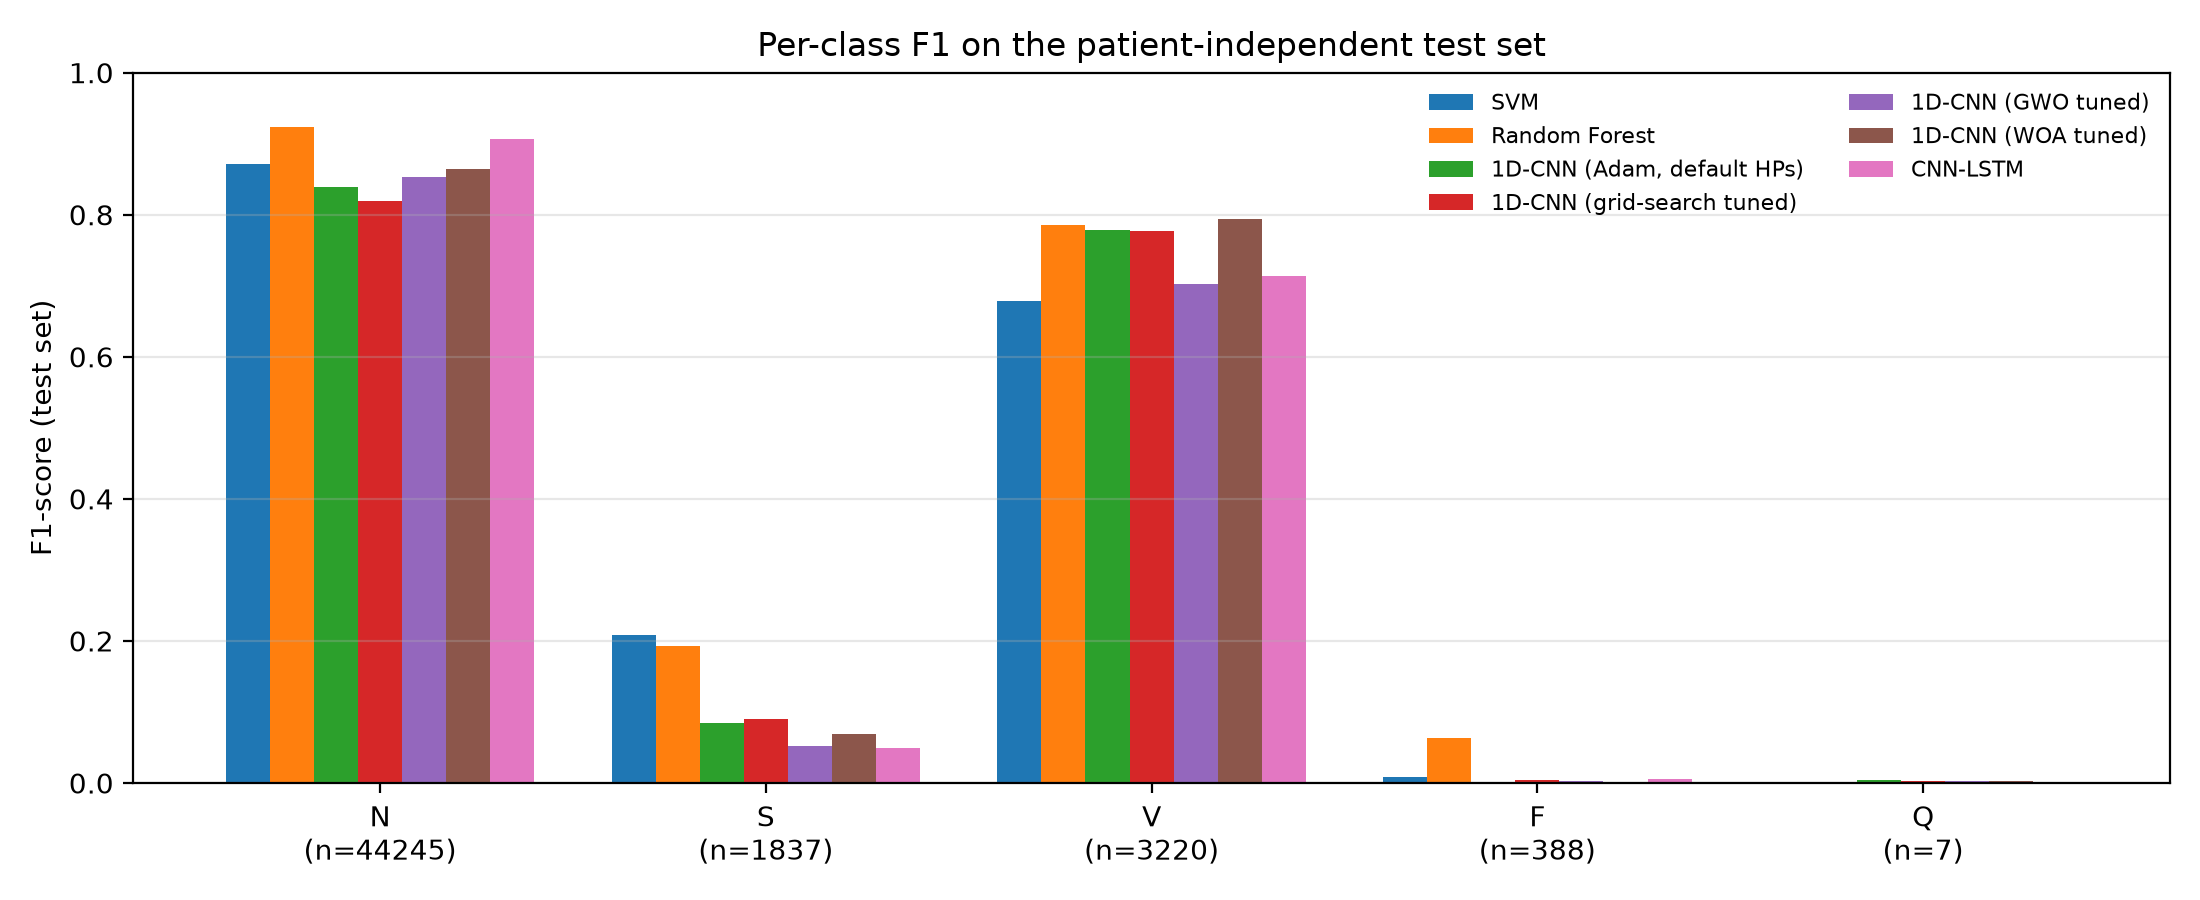
\includegraphics[width=\textwidth]{per_class_f1.png}
\caption{Per-class F1 of every model on the test set.}
\label{fig:f1}
\end{figure}

The Random Forest on hand-crafted features gives the best macro-F1 (0.393, or 0.491 without Q) of all models, ahead of the best deep model (WOA-tuned CNN, 0.346). It is the only model that detects a useful share of S beats (F1 0.19 against at most 0.09 for the networks) and has the best F class result (F1 0.06, recall 0.29). The reason is the RR-interval features: an S beat looks almost normal but arrives early, and the previous-RR and RR-ratio features describe exactly this timing, which a network that sees one 0.56 s window cannot measure. The same features were missing in the interim run of the Random Forest (macro-F1 0.31, S F1 0.00), so most of its improvement comes from them and from SMOTE. The SVM, trained on the same features, has the highest S-class F1 (0.21) and the second-best macro-F1 (0.353), but it labels 5,969 Normal beats as Fusion, which lowers its accuracy to 0.777. Both classical models show the same overfitting as the tuning experiment below: their cross-validated macro-F1 on the training data was 0.98--1.00 against 0.35--0.39 on the test patients, because the cross-validation folds contain beats of the same patients and SMOTE creates synthetic beats from neighbours that end up in different folds.

The deep models learn the shape of ventricular beats well without any hand-crafted features: the CNN variants reach a V-class F1 of 0.70--0.79, as high as the Random Forest (0.79). Ventricular beats have a wide, abnormally shaped QRS complex, which the convolutional filters learn directly from the waveform. The CNN-LSTM has the highest accuracy among the deep models (0.834) and the fewest false alarms on Normal beats among them (N recall 0.871, against 0.758 for the CNN): seeing the four preceding beats helps it confirm that a beat belongs to a regular normal rhythm. Its macro-F1 (0.335) is nevertheless no better than the single-beat CNN (0.342), because the gain on N is offset by more Normal beats wrongly labelled S (3,871) and a lower V precision (0.62). In principle the LSTM could learn the RR timing from the beat sequence, but each input window is centred on its R-peak, so the time between beats is not visible in the sequence of windows; only the shape of the neighbouring beats is.

\subsection{Error analysis}
Figure~\ref{fig:cm} shows the row-normalised confusion matrices; the counts are in \texttt{results/error\_analysis.txt}. Three error patterns are common to all models.

\begin{figure}[H]
\centering
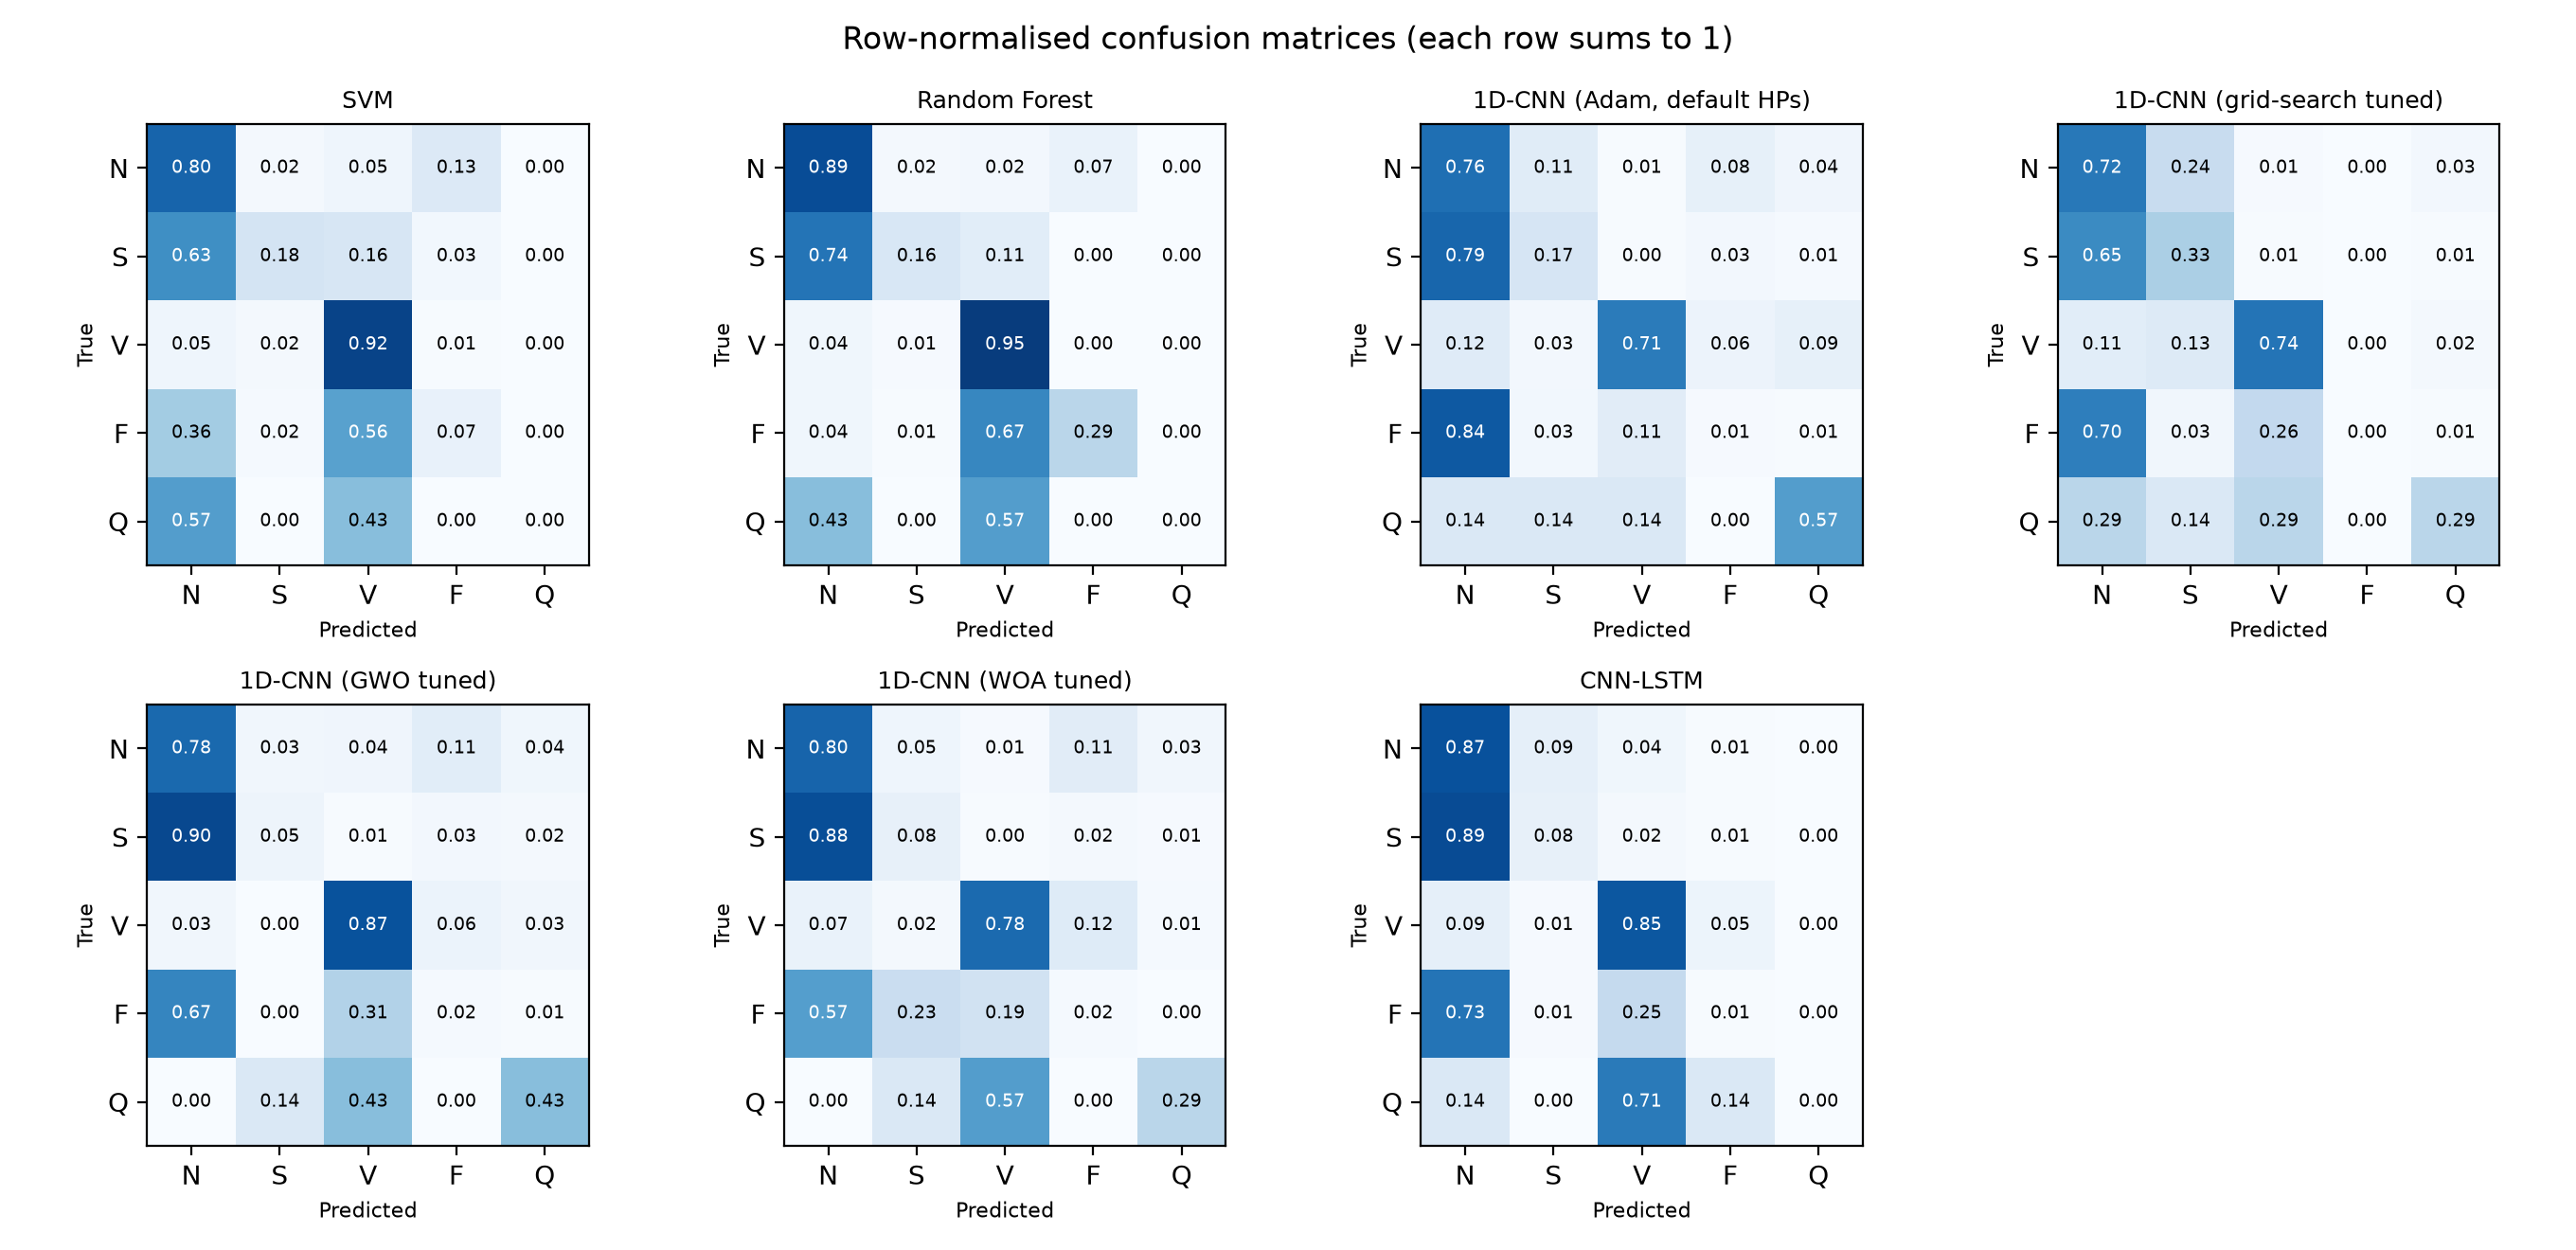
\includegraphics[width=\textwidth]{confusion_matrices.png}
\caption{Row-normalised confusion matrices (rows are true classes, each row sums to 1).}
\label{fig:cm}
\end{figure}

\begin{enumerate}
\item \textbf{S beats are classified as Normal.} Every model predicts most true S beats as N: from 63\% (SVM) to 90\% (GWO-tuned CNN). A supraventricular ectopic beat starts above the ventricles, so its QRS complex looks almost exactly like a normal one; what distinguishes it is that it arrives early. The networks receive only R-peak-centred windows and therefore never see this timing, and they miss 65--90\% of S beats. The SVM and Random Forest, which receive the RR intervals, miss the fewest (63\% and 74\%), but even with timing information most S beats are missed, because the prematurity of an S beat must be judged against the patient's own heart rate, and the training set contains only 944 S beats. In addition, the S class is concentrated in very few patients: 1,382 of the 1,837 test S beats (75\%) come from a single record (232), and 383 of the 944 training S beats come from record 209. The models therefore learn the S beats of a handful of training patients and are tested mostly on one different patient, whose beats they do not generalise to.
\item \textbf{Class weights cause many false alarms on Normal beats.} Balanced class weights give one Q training beat roughly 1,275 times the weight of an N beat. The networks therefore move part of the abundant N class into the rare classes: the untuned CNN labels 5,013 N beats as S, 3,659 as F and 1,733 as Q, and these errors make up 77\% of its mistakes. Because N is so large, even a few percent of N beats wrongly predicted is enough to make the precision of S, F and Q close to zero.
\item \textbf{Fusion beats are confused with V and N.} A fusion beat is a mix of a normal and a ventricular beat, so its shape lies between the two classes. The classical models predict most F beats as V (56--67\%), and the networks predict most of them as N (57--84\%), and F-class F1 is at most 0.013 for every model. 372 of the 414 training F beats come from one patient (record 208) and 362 of the 388 test F beats from another (record 213), so the F class is in effect learned from one patient and tested on a different one.
\end{enumerate}

The Q-class scores are not meaningful: with 7 test beats, one correct prediction changes Q recall by 0.14.

\subsection{Metaheuristic versus grid-search tuning}
Table~\ref{tab:tuning} and Figure~\ref{fig:tune} compare the four CNN variants.

\begin{table}[H]
\centering\small
\caption{1D-CNN tuning experiment. All tuners had the same budget of 36 short training runs.}
\label{tab:tuning}
\begin{tabular}{lrrrl}
\toprule
\textbf{Variant} & \textbf{Val. macro-F1} & \textbf{Test acc.} & \textbf{Test macro-F1} & \textbf{Selected hyperparameters} \\
\midrule
Default (Adam) & -- & 0.727 & 0.342 & lr $10^{-3}$, filters 32/64/128, kernel 7, dropout 0.3, dense 64 \\
Grid search & 0.462 & 0.703 & 0.339 & lr $10^{-3}$, filters 32/64/128, kernel 7, dropout 0.3, dense 64 \\
GWO & 0.627 & 0.751 & 0.323 & lr $5.5\times10^{-4}$, filters 78/156/312, kernel 11, dropout 0.16, dense 161 \\
WOA & 0.556 & 0.763 & 0.346 & lr $1.3\times10^{-4}$, filters 125/250/500, kernel 7, dropout 0.17, dense 75 \\
\bottomrule
\end{tabular}
\end{table}

\begin{figure}[H]
\centering
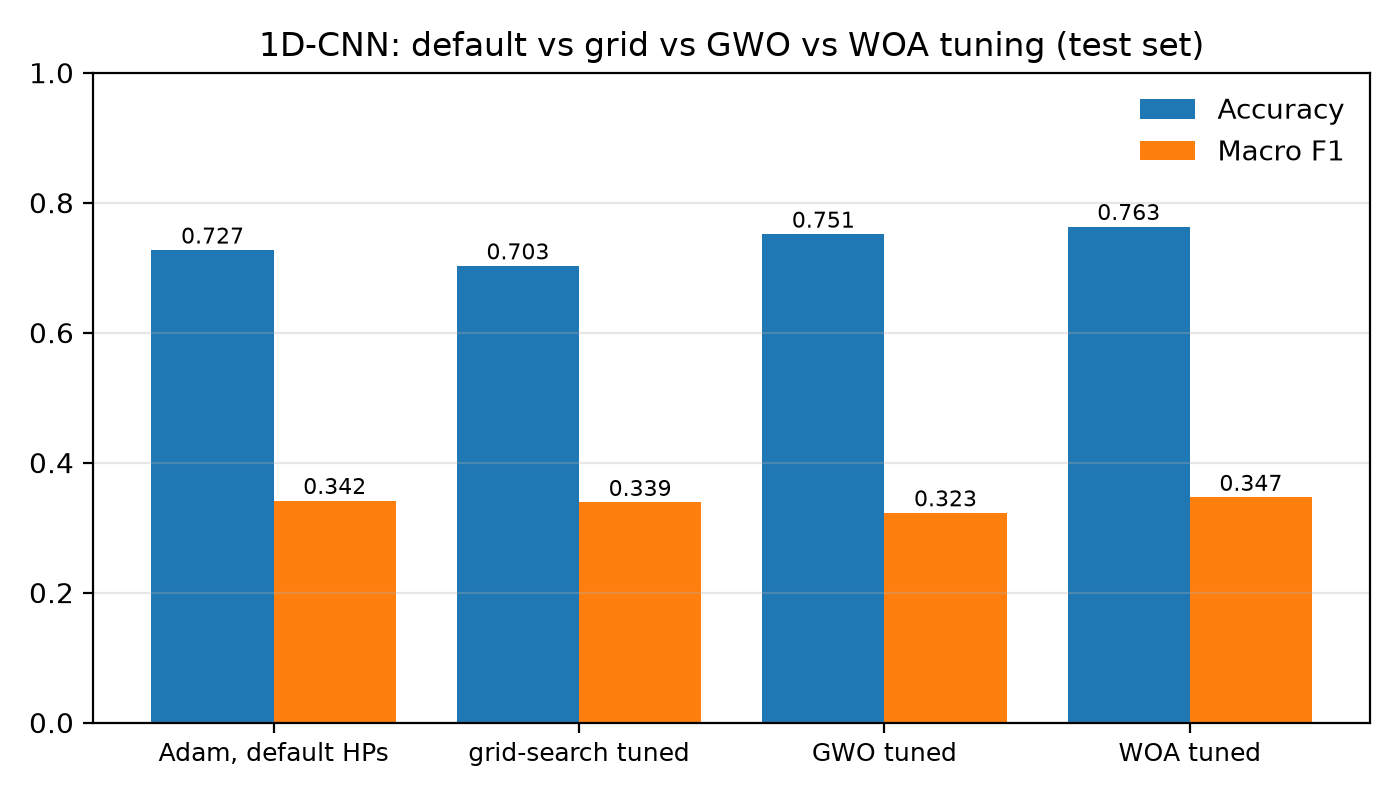
\includegraphics[width=0.7\textwidth]{tuning_comparison.png}
\caption{Test accuracy and macro-F1 of the four CNN variants.}
\label{fig:tune}
\end{figure}

GWO and WOA both found configurations with clearly higher validation macro-F1 than the best grid point (0.627 and 0.556 against 0.462), because their continuous search space also covers dropout, the dense layer size and larger networks, which the grid kept fixed. These gains did not carry over to the test set. WOA improved test macro-F1 by only about 0.005 over the untuned CNN and GWO was 0.019 worse, even though both raised accuracy by 2--4 points by predicting fewer S beats. The grid search selected exactly the default configuration, but its retrained model scored 0.024 lower in accuracy than the default run, which shows how much a single training run varies.

The cause is the validation set used during the search. It is a random 15\% of the training beats, so it contains beats from the same patients as the training data, while the test set contains new patients. The optimizers therefore select hyperparameters that fit the training patients well (GWO chose the largest model and the least dropout), which is the overfitting that the inter-patient protocol is designed to expose. The difference between configurations on the test set (0.323--0.346) is smaller than the variation between two runs of the same configuration. On this dataset, metaheuristic tuning is therefore not worth its cost: the search took 36 extra training runs per optimizer and gave no reliable improvement. A validation set made of separate training patients would be required to test the optimizers fairly.

\subsection{Comparison with published work}
Our scores are much lower than the 94--98\% accuracies reported in [3], [5], [14], but those studies use intra-patient splits or do not state their split. Under the inter-patient protocol, published S-class F1 values are in the range 0.5--0.6 [4], [12], and our models reach at most 0.09. The difference is mainly due to methods we did not use: those papers include explicit RR-interval normalisation per patient [12], sequence-to-sequence modelling with targeted resampling [21], or larger models trained with additional databases [4].

\subsection{Limitations}
\begin{enumerate}
\item \textbf{Early stopping on the test set.} The CNN, its tuned retrains and the CNN-LSTM used the test set as the validation set for early stopping and learning-rate reduction. This makes their test scores slightly optimistic. The SVM and Random Forest do not have this problem. Fixing it requires holding out separate training patients as a validation set and rerunning the networks on a GPU.
\item \textbf{Single run per model.} Differences of a few points between models are within the variation between runs (for example, the default CNN gave 0.727 and 0.733 accuracy in two runs), so they should not be read as significant.
\item \textbf{The CNN-LSTM is scored on 88 fewer test beats} (the first four beats of each record), which slightly changes its test set.
\item \textbf{Q class.} With 8 training and 7 test beats, Q cannot be learned or evaluated; macro-F1 without Q is reported for this reason.
\end{enumerate}

%=====================================================================
\section{Conclusion}
We compared an SVM, a Random Forest, a 1D-CNN and a CNN-LSTM for five-class ECG beat classification on MIT-BIH under one patient-independent protocol, and tested GWO and WOA against a grid search for tuning the CNN. The Random Forest with RR-interval features and SMOTE gave the best accuracy (0.860) and macro-F1 (0.393), and the two classical models were the only ones to detect a meaningful share of supraventricular beats (F1 about 0.2), because the RR intervals capture the early timing of these beats. The deep models detect ventricular beats better, and the CNN-LSTM's beat-sequence context reduces false alarms on normal beats. However, no model reliably detects supraventricular or fusion beats in unseen patients, so macro-F1 stays below 0.40 for every model. Metaheuristic tuning improved validation scores but not test performance, because the validation beats came from the training patients. Under a strict inter-patient protocol, the number of training patients and the class imbalance limit performance more than the choice of model family or tuner.

\section{Future Work}
\begin{itemize}
\item Use a patient-wise validation split (separate DS1 records) for early stopping and for the GWO/WOA fitness function, and repeat every model with at least three seeds.
\item Give the deep models RR-interval inputs normalised per patient, which the literature identifies as the key cue for S beats [12].
\item Replace plain class weights with focal loss or a resampling of the minority classes at the batch level, to reduce false alarms on N beats.
\item Add the MIT-BIH Supraventricular Arrhythmia Database or INCART to increase the number of S and F examples and patients.
\item Evaluate an attention-based model as a fourth architecture family.
\end{itemize}

\section*{Acknowledgement}
We thank the course faculty of ICT 4442 for their guidance, PhysioNet for providing the MIT-BIH Arrhythmia Database free of charge, and Kaggle for the free GPU time used to train the neural networks.

\section*{Use of External Tools and LLM Assistance}
As required by the academic integrity policy, we state where an LLM was used. Claude Code (Anthropic) was used to: generate the first versions of \texttt{src/cnn\_model.py}, \texttt{src/cnn\_lstm\_model.py}, and \texttt{src/metaheuristic\_tuning.py}; add the RR-interval features, SMOTE and grid search to \texttt{src/preprocessing.py} and \texttt{src/svm\_baseline.py}; write \texttt{src/compare\_results.py}, \texttt{README.md} and the Kaggle notebooks; run the final SVM/Random Forest experiment; and draft this report from the repository code and result files. All numbers in this report are taken from the result files produced by our runs. The first version of the repository contains a \texttt{.github/copilot-instructions.md} file, which suggests GitHub Copilot was used for the first preprocessing pipeline and baseline [Chinmai to confirm]. [Pranshu Singh to state whether an LLM was used for \texttt{src/grid\_search\_tuning.py}; all members to confirm that each methodology section was rewritten by its owner.] Every member is responsible for understanding and explaining the code and results of their assigned model.

%=====================================================================
\begin{thebibliography}{99}
\bibitem{r1} G. B. Moody and R. G. Mark, ``The impact of the MIT-BIH Arrhythmia Database,'' \textit{IEEE Engineering in Medicine and Biology Magazine}, vol. 20, no. 3, pp. 45--50, 2001.
\bibitem{r2} A. L. Goldberger et al., ``PhysioBank, PhysioToolkit, and PhysioNet: Components of a new research resource for complex physiologic signals,'' \textit{Circulation}, vol. 101, no. 23, pp. e215--e220, 2000.
\bibitem{r3} M. M. R. Khan, M. A. B. Siddique, S. Sakib, A. Aziz, A. K. Tanzeem, and Z. Hossain, ``Electrocardiogram heartbeat classification using convolutional neural networks for the detection of cardiac arrhythmia,'' in \textit{Proc. 4th Int. Conf. I-SMAC}, IEEE, 2020 (arXiv:2010.04086).
\bibitem{r4} L. Guo, G. Sim, and B. Matuszewski, ``Inter-patient ECG classification with convolutional and recurrent neural networks,'' arXiv preprint arXiv:1810.04121, 2018.
\bibitem{r5} N. Alamatsaz, L. Tabatabaei, M. Yazdchi, H. Payan, N. Alamatsaz, and F. Nasimi, ``A lightweight hybrid CNN-LSTM model for ECG-based arrhythmia detection,'' arXiv preprint arXiv:2209.00988, 2022.
\bibitem{r6} R. Nikandish, J. He, and B. Haghi, ``Multi-feature fusion and compressed Bi-LSTM for memory-efficient heartbeat classification on wearable devices,'' arXiv preprint arXiv:2405.15312, 2024.
\bibitem{r7} \"{O}. Yildirim, ``A novel wavelet sequence based on deep bidirectional LSTM network model for ECG signal classification,'' \textit{Computers in Biology and Medicine}, vol. 96, pp. 189--202, 2018.
\bibitem{r8} A. Ben Slama, Y. Amri, A. Fnaiech, and H. Sahli, ``Automated ECG arrhythmia classification using hybrid CNN-SVM architectures,'' \textit{Journal of Electronic Science and Technology}, vol. 23, no. 3, p. 100316, 2025.
\bibitem{r9} S. Mirjalili, S. M. Mirjalili, and A. Lewis, ``Grey Wolf Optimizer,'' \textit{Advances in Engineering Software}, vol. 69, pp. 46--61, 2014.
\bibitem{r10} S. Mirjalili and A. Lewis, ``The Whale Optimization Algorithm,'' \textit{Advances in Engineering Software}, vol. 95, pp. 51--67, 2016.
\bibitem{r11} Q. S. Hamad, H. Samma, and S. A. Suandi, ``Optimization of convolutional neural network hyperparameter for medical image diagnosis using metaheuristic algorithms: a short recent review (2019--2022),'' arXiv preprint arXiv:2412.17956, 2024.
\bibitem{r12} P. de Chazal, M. O'Dwyer, and R. B. Reilly, ``Automatic classification of heartbeats using ECG morphology and heartbeat interval features,'' \textit{IEEE Transactions on Biomedical Engineering}, vol. 51, no. 7, pp. 1196--1206, 2004.
\bibitem{r13} S. Kiranyaz, T. Ince, and M. Gabbouj, ``Real-time patient-specific ECG classification by 1-D convolutional neural networks,'' \textit{IEEE Transactions on Biomedical Engineering}, vol. 63, no. 3, pp. 664--675, 2016.
\bibitem{r14} U. R. Acharya, S. L. Oh, Y. Hagiwara, J. H. Tan, M. Adam, A. Gertych, and R. S. Tan, ``A deep convolutional neural network model to classify heartbeats,'' \textit{Computers in Biology and Medicine}, vol. 89, pp. 389--396, 2017.
\bibitem{r15} S. Hochreiter and J. Schmidhuber, ``Long short-term memory,'' \textit{Neural Computation}, vol. 9, no. 8, pp. 1735--1780, 1997.
\bibitem{r16} G. Silva, P. Silva, G. Moreira, V. Freitas, J. Gertrudes, and E. Luz, ``A systematic review of ECG arrhythmia classification: adherence to standards, fair evaluation, and embedded feasibility,'' arXiv preprint arXiv:2503.07276, 2025.
\bibitem{r17} H. M. Mohammed, S. U. Umar, and T. A. Rashid, ``A systematic and meta-analysis survey of whale optimization algorithm,'' \textit{Computational Intelligence and Neuroscience}, vol. 2019, Art. no. 8718571, 2019.
\bibitem{r18} ANSI/AAMI EC57:2012, \textit{Testing and Reporting Performance Results of Cardiac Rhythm and ST Segment Measurement Algorithms}, Association for the Advancement of Medical Instrumentation, 2012.
\bibitem{r19} C. Cortes and V. Vapnik, ``Support-vector networks,'' \textit{Machine Learning}, vol. 20, no. 3, pp. 273--297, 1995.
\bibitem{r20} L. Breiman, ``Random forests,'' \textit{Machine Learning}, vol. 45, no. 1, pp. 5--32, 2001.
\bibitem{r21} S. Mousavi, F. Afghah, and U. R. Acharya, ``Inter- and intra-patient ECG heartbeat classification for arrhythmia detection: a sequence to sequence deep learning approach,'' arXiv preprint arXiv:1812.07421, 2018.
\bibitem{r22} N. V. Chawla, K. W. Bowyer, L. O. Hall, and W. P. Kegelmeyer, ``SMOTE: Synthetic minority over-sampling technique,'' \textit{Journal of Artificial Intelligence Research}, vol. 16, pp. 321--357, 2002.
\bibitem{r23} D. P. Kingma and J. Ba, ``Adam: A method for stochastic optimization,'' in \textit{Proc. ICLR}, 2015 (arXiv:1412.6980).
\end{thebibliography}

%=====================================================================
\newpage
\section*{Individual Contribution Statement}
\addcontentsline{toc}{section}{Individual Contribution Statement}
All three members contributed equally to the project. The table summarises each member's main areas of work.

\begin{table}[H]
\centering\small
\begin{tabular}{p{3.2cm}p{10.3cm}p{1.8cm}}
\toprule
\textbf{Member} & \textbf{Main contributions} & \textbf{Share} \
\midrule
Tanush Ralhan & 1D-CNN and CNN-LSTM implementation, GWO/WOA tuning code, RR-interval features and SMOTE, final SVM/Random Forest run, comparison table, error analysis and figures, final report & Equal \
Pranshu Singh & Grid-search control experiment, Kaggle training runs for the 1D-CNN, grid-search, GWO and WOA tuned models and their results & Equal \
Chinmai & Repository setup, dataset download script, initial preprocessing pipeline, first SVM/Random Forest baseline, synopsis & Equal \
\bottomrule
\end{tabular}
\end{table}

\vspace{0.8cm}
\noindent\textbf{Signed by all members:}\\[1.2cm]
\begin{tabular}{p{5cm}p{5cm}p{5cm}}
\rule{4.5cm}{0.4pt} & \rule{4.5cm}{0.4pt} & \rule{4.5cm}{0.4pt} \\
Tanush Ralhan (230911564) & Pranshu Singh & Chinmai (230911318) \\
Date: & Date: & Date: \\
\end{tabular}

\end{document}
